\documentclass{beamer}
\input{common.tex}

\title{Tutorium 14: Bytecode \& Wiederholung}
% \subtitle{}
\author{David Kaufmann}
\institute{Tutorium Programmierparadigmen am KIT}
\date{15. Februar 2023}

\begin{document}
\begin{frame}
	\titlepage
\end{frame}

\subsection{AST Erzeugung}

\begin{frame}{Aufgabe}
    Wir bauen den Parser von letzter Woche weiter...
    \begin{columns}
        \begin{column}{0.5 \textwidth}
            \begin{itemize}
                \item Zu jeder Kategorie eine Klasse
                \item Jeder Blatttyp und innerer Knoten ein Konstruktor
                \item Unterklassen für Kategorie sind Alternativen
                \item Baum soll links-assoziativ sein
            \end{itemize}
        \end{column}
        \begin{column}{0.5 \textwidth}
           $$(a+b+c)/a$$
           \begin{figure}
               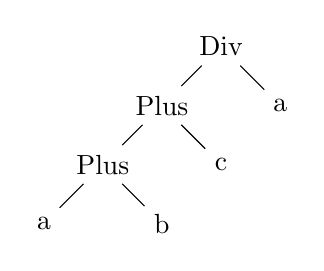
\begin{tikzpicture}[
                  level distance=7.5mm,
                  sibling distance=15mm
                ]
                  \node {Div}
                    child {
                      node {Plus}
                        child {
                          node {Plus}
                            child {node {a}}
                            child {node {b}}
                        }
                        child {node {c}}
                    }
                    child {node {a}}
                  ;
                \end{tikzpicture}
           \end{figure}
       \end{column}
    \end{columns}
\end{frame}

\begin{frame}{Aufgabe}
	\footnotesize
	\begin{align*}
		E     \to & \;\; T \;\; EList\\
		EList \to & \;\; \epsilon \mid \textrm{\texttt{+}} \;\; T \;\; EList \mid \textrm{\texttt{-}} \;\; T \;\; EList\\
		T     \to & \;\; F \;\; TList\\
		TList \to & \;\; \epsilon \mid \textrm{\texttt{*}} \;\; F \;\; TList \mid \textrm{\texttt{/}} \;\; F \;\; TList\\
		F \to & \;\; \textrm{\texttt{num}} \; | \; \textrm{\texttt{(}} \;\; E \;\; \textrm{\texttt{)}}
	\end{align*}
	\begin{itemize}
            \item Der Parser soll einen AST zurückgeben
		\item Verwendet die Klassen aus \texttt{./demos/compiler/Exp.java}
            \item Der Baum soll wie auf letzter Folie aussehen
	\end{itemize}
\end{frame}

\subsection{Semantische Analyse/Optimierung}

\begin{frame}{Semantische Analyse}
	\begin{itemize}
		\item PP beschäftigt sich (bis auf Typinferenz) nur kurz mit semantischer Analyse
		\item Typchecks/-inferenz, Namensanalyse
		\item $\leadsto$ weiterführende (Master-)Vorlesungen am IPD
	\end{itemize}
\end{frame}

\section{Java-Bytecode}

\begin{frame}{wichtige Befehle}
    \begin{itemize}
        \item \texttt{X\_const\_i}: läd Konstante für $i \in [-1,5]$ auf den Stack
        \item \texttt{bipush <i>}: läd Konstante für $i \in [-127,128]$
        \item \texttt{Xload <x>, Xstore <x>}: lesen/schreiben von lokalen Variablen (für Integer gibt es eigenen Opcode für $x \in [0,3]$)
        \item \texttt{Xmul, Xadd,...}: Arithmetik
    \end{itemize}
\end{frame}

\begin{frame}{Beispiel}
    \begin{columns}
        \begin{column}
            
        \end{column}
    \end{columns}
\end{frame}

\section{Ende}

\begin{frame}{Letzte Folie}
  \begin{itemize}
    \item ÜB-Korrekturen: Blatt 13 korregiere ich noch
    \item Klausur: 31.03.2023, 11:30
    \item Tutoriumsfolien, -code, etc.: \href{https://github.com/KaufmannDavid/propa-tut}{github.com/KaufmannDavid/propa-tut}
    \item Fragen auch gerne an \texttt{david.kaufmann@student.kit.edu} :)
  \end{itemize}

  \vfill

  Danke fürs Kommen und eine erfolgreiche Prüfungsphase!
\end{frame}
\end{document}